\documentclass{beamer}
\usepackage{beamerthemesplit}
\usepackage[utf8]{inputenc}
\usepackage[portuguese]{babel}
\usepackage{graphicx}
\usepackage{tikz}
\usepackage{animate}

\newsavebox{\picbox}

\newcommand{\cutpic}[3]{
  \savebox{\picbox}{\includegraphics[width=#2]{#3}}
  \tikz\node [draw, rounded corners=#1, line width=4pt,
    color=white, minimum width=\wd\picbox,
    minimum height=\ht\picbox, path picture={
        \node at (path picture bounding box.center) {
          \usebox{\picbox}};
      }] {};
}

% Beamer config
\usetheme{Copenhagen}
\usecolortheme{dolphin}
\beamertemplatenavigationsymbolsempty

\mode<presentation>{}



\title[Eventos no DOM]{Eventos no DOM}
\author{Davi Valadares Rodrigues Feliciano}
\institute{Driven Education}
\date{03 de fevereiro de 2023}

\begin{document}

\begin{frame}
  \maketitle
\end{frame}

\begin{frame}{O que são eventos?}
  \begin{block}{No contexto geral}
    \begin{itemize}
      \item É uma ocorrência reconhecível por \textit{software}, um sinal emitido que
            pode ser identificado e interpretado
      \item Normalmente originada assincronamente por uma fonte externa
      \item Após interpretar um evento, um \textit{software} pode lidar de acordo com o
            tipo do evento em sua execução
    \end{itemize}
  \end{block}
  \begin{exampleblock}{Exemplos}
    \begin{itemize}
      \item Exemplos de fontes são o usuário por meio de periféricos ou mesmo
            outros \textit{softwares}
      \item O próprio modelo de \textit{runtime} do JavaScript consiste em um loop de
            eventos
    \end{itemize}
  \end{exampleblock}
\end{frame}

\begin{frame}{O que são eventos?}
  \begin{block}{No contexto do DOM}
    \begin{itemize}
      \item Eventos são disparados frequentemente ao longo do uso de uma página
            o \textit{browser}
      \item Esses eventos normalmente estão acoplados a um ou múltiplos
            elementos
    \end{itemize}
  \end{block}
  \begin{exampleblock}{Exemplos de Eventos}
    \begin{columns}
      \begin{column}{0.45\textwidth}
        \begin{itemize}
          \item Clicar em um elemento
          \item Pressionar teclas
          \item \textit{Drag and drop}
          \item \textit{Scroll}
        \end{itemize}
      \end{column}
      \begin{column}{0.5\textwidth}
        \begin{itemize}
          \item Copiar, cortar e colar
          \item \textit{Reset} ou \textit{submit} de \textit{forms}
          \item No carregamento da página
          \item Redimensionar a janela
        \end{itemize}
      \end{column}
    \end{columns}
  \end{exampleblock}
\end{frame}

\begin{frame}{O que são eventos?}
  \begin{block}{No contexto do DOM}
    \begin{itemize}
      \item Para reagir à ocorrência desses eventos, devemos capturá-los de
            alguma forma
      \item Eventos não capturados disparam comportamentos padrões
      \item Para isso usamos \textit{event listeners} e \textit{event handlers}
      \item \textit{Event listeners}, como o próprio nome diz, quando ativados,
            aguardam o disparo de um determinado evento
      \item Quando este ocorre, o \textit{event handler}, que é uma função
            previamente definida é executado
    \end{itemize}
  \end{block}
\end{frame}

\begin{frame}[fragile]{Criando \textit{event listeners} no JavaScript}
  \begin{itemize}
    \item Para criar um \textit{event listener} usamos o método addEventListener
          de objetos do tipo Element
    \item Passamos como primeiro parâmetro uma string identificadora do tipo de
          evento a ser capturado
    \item Como segundo argumento, passamos uma função de \textit{callback} que
          será executada em cada ocorrência do evento
    \item Para essa função de \textit{callback} é passado uma instância de um
          objeto Event
  \end{itemize}
  \begin{block}{O que é uma função de \textit{callback}?}
    \begin{itemize}
      \item É uma função passada como argumento para outra função
      \item Será chamada em algum momento na execução da última
    \end{itemize}
  \end{block}
\end{frame}

\begin{frame}{Objetos Event}
  \begin{figure}
    \centering
    \cutpic{.2cm}{0.8\textwidth}{images/event_listener.png}
  \end{figure}
  \begin{table}
    \centering
    \begin{tabular}{|l|p{0.6\textwidth}|}
      \hline
      Event.type          & Uma string identificando o tipo do evento                                                 \\ \hline
      Event.timeStamp     & O momento em que o evento ocorreu, em milissegundos, em relação ao carregamento da página \\ \hline
      Event.currentTarget & Uma referência ao elemento ao qual o listener foi acoplado                                \\ \hline
      Event.target        & Uma referência ao elemento no qual o evento teve origem (\textit{event bubbling})         \\ \hline
    \end{tabular}
  \end{table}
\end{frame}

\begin{frame}{Objetos Event}
  \begin{columns}
    \begin{column}{0.6\textwidth}
      \begin{figure}
        \centering
        \cutpic{.2cm}{\textwidth}{images/examples.png}
      \end{figure}
    \end{column}
    \begin{column}{0.3\textwidth}
      \centering
      \animategraphics[loop,autoplay,width=\textwidth]{10}{images/driveneats_frames/driveneats_events-}{0}{139}
    \end{column}
  \end{columns}
\end{frame}

\begin{frame}{Event Bubbling}
  \begin{columns}
    \begin{column}{0.4\textwidth}
      \begin{itemize}
        \item Quando um evento é criado, ele se propaga pelos níveis superiores da
              árvore de elementos do DOM, até chegar ao elemento raiz
        \item Isso significa que mesmo um elemento não tendo \textit{event listeners}
              acoplados ainda pode disparar \textit{event handlers} em seus pais
      \end{itemize}
    \end{column}
    \begin{column}{0.6\textwidth}
      \begin{figure}
        \centering
        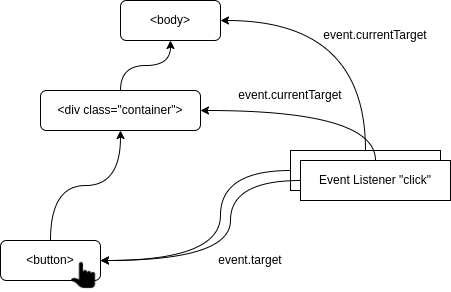
\includegraphics[width=\textwidth]{images/event_bubbling.png}
      \end{figure}
    \end{column}
  \end{columns}
\end{frame}

\begin{frame}{Event Bubbling}
  \begin{itemize}
    \item Como prevenir esse comportamento quando indesejado? Com uma chamada ao
          método event.stopPropagation
  \end{itemize}
  \begin{figure}
    \centering
    \cutpic{.2cm}{0.8\textwidth}{images/stop_propagation_html.png}
  \end{figure}
  \begin{figure}
    \centering
    \cutpic{.2cm}{0.8\textwidth}{images/stop_propagation_js.png}
  \end{figure}
\end{frame}

\begin{frame}{addEventListener vs. onclick}
  \begin{itemize}
    \item É possível adicionar múltiplos \textit{event listeners} a um único
          elemento
    \item Como citado, existem vários tipos de evento que não são acessíveis em
          atributos do HTML
    \item \textit{Event listener} possibilita o acesso a propriedades do evento
          por meio de objetos do tipo Event, o que pode ser útil em diversas
          aplicações
  \end{itemize}
\end{frame}

\end{document}